\documentclass[10pt, letterpaper]{article}

\usepackage{tikz} 
\usepackage{pgfplots}
\pgfplotsset{compat=1.9}
\usetikzlibrary{arrows,shapes,automata,backgrounds,petri,fit,decorations.pathmorphing, calc}

\begin{document}


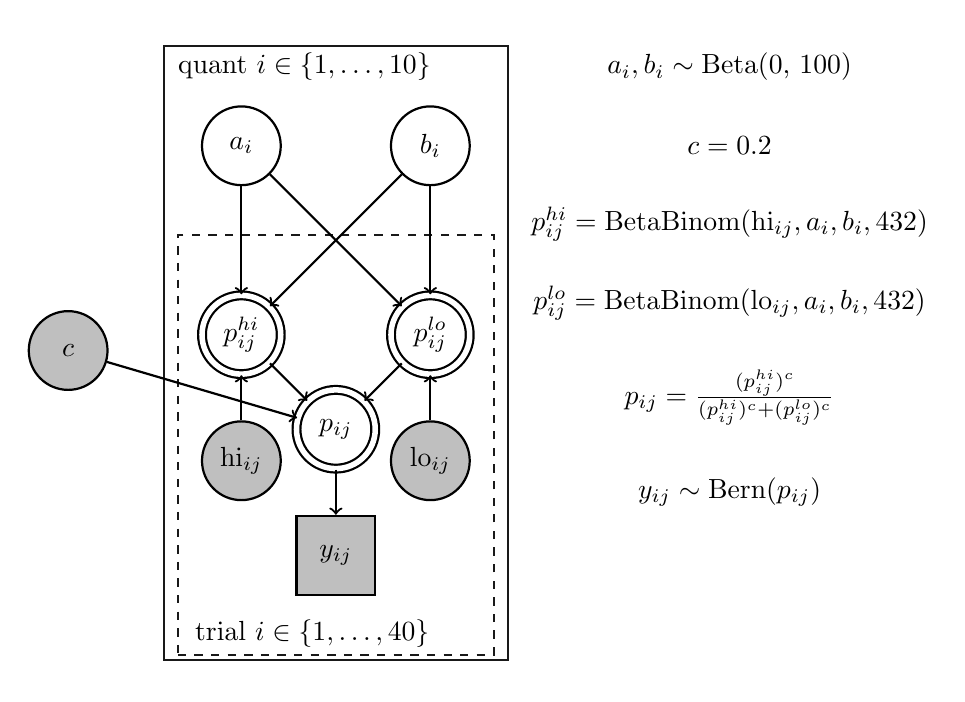
\begin{tikzpicture}[node distance = 2.4cm, double distance = 2pt, minimum size=1cm, thick]
  \node[circle, draw=black] (a) {$a_i$};
  \node[circle, draw=black, right of = a] (b) {$b_i$};
  
  \node[circle, draw=black, below of = a, double] (phi) {$p^{hi}_{ij}$};
  \node[circle, draw=black, right of = phi, double] (plo) {$p^{lo}_{ij}$};
  \node[circle, draw=black, below of = phi, right of = phi, double, node distance = 1.2cm] (p) {$p_{ij}$};
  
  \node[rectangle, draw=black, fill=lightgray, below of = p, node distance = 1.6cm] (y) {$y_{ij}$};
  
  \node[circle, draw=black, fill=lightgray, left of = y, node distance = 1.2cm, yshift = 1.2cm]
  (hi) {$\mbox{hi}_{ij}$};
  
  \node[circle, draw=black, fill=lightgray, right of = y, node distance = 1.2cm, yshift = 1.2cm]
  (lo) {$\mbox{lo}_{ij}$};
  
  \node[circle, draw=black, fill=lightgray, left of = p, node distance = 3.4cm, yshift = 1cm] (c) {$c$};
  
  
  \draw[->] (a)--(phi);
  \draw[->] (a)--(plo);
  
  \draw[->] (b)--(phi);
  \draw[->] (b)--(plo);
  
  \draw[->] (phi)--(p);
  \draw[->] (plo)--(p);
  \draw[->] (hi)--(phi);
  \draw[->] (lo)--(plo);
  \draw[->] (p)--(y);
  \draw[->] (c)--(p);
  
   \begin{pgfonlayer}{background}
       \node [thick,
              draw=black!90,fit={($(y.south)+(0,-20pt)$) 
                                 ($(a.west)+(-10pt,-10pt)$) 
                                 ($(a.north)+(0,18pt)$) 
                                 ($(b.east)+(+10pt,+10pt)$)}] {};
    \end{pgfonlayer}
    
    \node[above of = a, node distance = 1cm] (QuantAnchor) {};
    \node[right of = QuantAnchor, node distance = .8cm] (QuantLabel) {quant $i \in \{1, \ldots, 10\}$};
    
   \begin{pgfonlayer}{background}
       \node [thick, dashed,
              draw=black!90,fit={($(y.south)+(0,-18pt)$) 
                                 ($(phi.west)+(-5pt,-5pt)$) 
                                 ($(phi.north)+(0,18pt)$) 
                                 ($(plo.east)+(+5pt,+5pt)$)}] {};
    \end{pgfonlayer}
    
    \node[below of = y, node distance = 1cm] (TrialAnchor) {};
    \node[left of = TrialAnchor, node distance = .3cm] (TrialLabel) {trial $i \in \{1, \ldots, 40\}$};
  
  
    \begin{scope}[xshift = 6.2cm, node distance = 1cm]
    
  
        \node[] at(0, 1) (a) {$a_i, b_i \sim \mbox{Beta(0, 100)}$};
  
        \node[below of = a] at(0,1) (c) {$c = 0.2$};
        
        \node[below of = c] (phi)
        {$p^{hi}_{ij} = \mbox{BetaBinom}(\mbox{hi}_{ij}, a_i, b_i, 432)$};
        
        \node[below of = phi] (plo)
        {$p^{lo}_{ij} = \mbox{BetaBinom}(\mbox{lo}_{ij}, a_i, b_i, 432)$};
        
        \node[below of = plo, node distance = 1.2cm] (p)
        {$p_{ij} = \frac{(p^{hi}_{ij})^c}{(p^{hi}_{ij})^c + (p^{lo}_{ij})^c}$};
        
        \node[below of = p, node distance = 1.2cm] (yij) {$y_{ij} \sim \mbox{Bern(}p_{ij})$};
        
    \end{scope}
    
\end{tikzpicture}

\end{document}